% !TeX spellcheck = en_GB
% !TeX program = pdflatex
%
% LuxSleek-CV 1.1 LaTeX template
% Author: Andreï V. Kostyrka, University of Luxembourg
%
% 1.1: added tracking and letter-spacing for prettier lower caps, added `~` for language levels
% 1.0: initial release
%
% This template fills the gap in the available variety of templates
% by proposing something that is not a custom class, not using any
% hard-coded settings deeply hidden in style files, and provides
% a handful of custom command definitions that are as transparent as it gets.
% Developed at the University of Luxembourg.
%
% *NOTHING IS HARCODED, and never should be.*
%
% Target audience: applicants in the IT industry, or business in general
%
% The main strength of this template is, it explicitly showcases how
% to break the flow of text to achieve the most flexible right alignment
% of dates for multiple configurations.

\documentclass[11pt, a4paper]{article} 

\usepackage[T1]{fontenc}     % We are using pdfLaTeX,
\usepackage[utf8]{inputenc}  % hence this preparation
\usepackage[british]{babel}  
\usepackage[left = 0mm, right = 0mm, top = 0mm, bottom = 0mm]{geometry}
\usepackage[stretch = 25, shrink = 25, tracking=true, letterspace=30]{microtype}  
\usepackage{graphicx}        % To insert pictures
\usepackage{xcolor}          % To add colour to the document
\usepackage{marvosym}        % Provides icons for the contact details

\usepackage{enumitem}        % To redefine spacing in lists
\setlist{parsep = 0pt, topsep = 0pt, partopsep = 1pt, itemsep = 1pt, leftmargin = 6mm}

\usepackage{FiraSans}        % Change this to use any font, but keep it simple
\renewcommand{\familydefault}{\sfdefault}

\definecolor{cvblue}{HTML}{304263}

%%%%%%% USER COMMAND DEFINITIONS %%%%%%%%%%%%%%%%%%%%%%%%%%%
% These are the real workhorses of this template
\newcommand{\dates}[1]{\hfill\mbox{\textbf{#1}}} % Bold stuff that doesn’t got broken into lines
\newcommand{\is}{\par\vskip.5ex plus .4ex} % Item spacing
\newcommand{\smaller}[1]{{\small$\diamond$\ #1}}
\newcommand{\headleft}[1]{\vspace*{3ex}\textsc{\textbf{#1}}\par%
    \vspace*{-1.5ex}\hrulefill\par\vspace*{0.7ex}}
\newcommand{\headright}[1]{\vspace*{2.5ex}\textsc{\Large\color{cvblue}#1}\par%
     \vspace*{-2ex}{\color{cvblue}\hrulefill}\par}
%%%%%%%%%%%%%%%%%%%%%%%%%%%%%%%%%%%%%%%%%%%%%%%%%%%%%%%%%%%%

\usepackage[colorlinks = true, urlcolor = white, linkcolor = white]{hyperref}

\begin{document}

% Style definitions -- killing the unnecessary space and adding the skips explicitly
\setlength{\topskip}{0pt}
\setlength{\parindent}{0pt}
\setlength{\parskip}{0pt}
\setlength{\fboxsep}{0pt}
\pagestyle{empty}
\raggedbottom

\begin{minipage}[t]{0.33\textwidth} %% Left column -- outer definition
%  Left column -- top dark rectangle
\colorbox{cvblue}{\begin{minipage}[t][5mm][t]{\textwidth}\null\hfill\null\end{minipage}}

\vspace{-.2ex} % Eliminates the small gap
\colorbox{cvblue!90}{\color{white}  %% LEFT BOX
\kern0.09\textwidth\relax% Left margin provided explicitly
\begin{minipage}[t][293mm][t]{0.82\textwidth}
\raggedright
\vspace*{2.5ex}

\Large Senior Software Engineer \textbf{\textsc{Ludovic Aubert}} \normalsize 

% Centering without extra vertical spacing
\null\hfill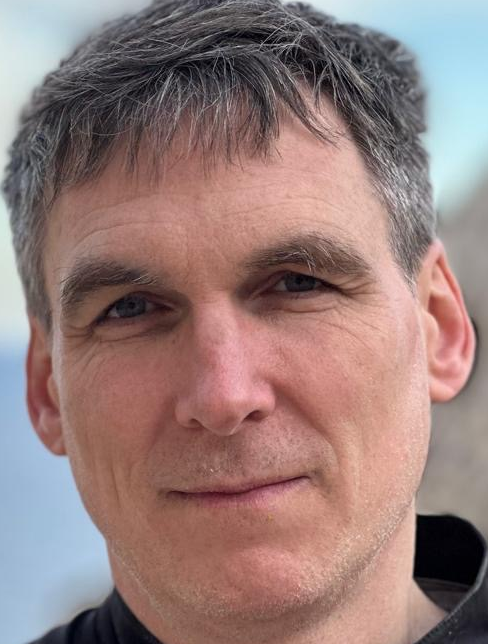
\includegraphics[width=0.65\textwidth]{lax.png}\hfill\null

\vspace*{0.5ex} % Extra space after the picture

\headleft{Projet}
Je suis ingénieur diplômé de l'École Centrale de Paris et je combine une solide formation en mathématiques avec 25 ans d'expérience dans des projets diversifiés de logiciels et de data. Au début de ma carrière, j'ai principalement travaillé sur des projets en C++, dont certains nécessitaient la conception d'algorithmes. Dans un deuxième temps, j'ai principalement travaillé sur des projets liés aux données. Je suis à la recherche de projets complexes et critiques, utilisant un mélange de données, de logiciels et de web.

\headleft{Contact}
\small % To fit more content
\MVAt\ {\small ludo.aubert@gmail.com} \\[0.4ex]
\Mobilefone\ 06\,68\,40\,98\,26\ \\[0.5ex]
\Mundus\ \href{https://github.com/ludoaubert}{github.com/ludoaubert} \\[0.1ex]

\headleft{Langues}
\textbf{Francais}~(native), \textbf{Espagnol}~(B1), \textbf{Allemand}~(C2), \textbf{Anglais}~(C2)

\headleft{Compétences}
\begin{itemize}
\item C++, SQL, CSS
\item Javascript, JSON, HTML
\item SQL Server, PostgreSQL, Oracle
\item NodeJS
\item Communication and team collaboration
\end{itemize} 

\end{minipage}%
\kern0.09\textwidth\relax%%Right margin provided explicitly to stretch the colourbox
}
\end{minipage}% Right column
\hskip2.5em% Left margin for the white area
\begin{minipage}[t]{0.56\textwidth}
\setlength{\parskip}{0.8ex}% Adds spaces between paragraphs; use \\ to add new lines without this space. Shrink this amount to fit more data vertically

\vspace{2ex}

\headright{Réalisations}

\textsc{Senior software engineer} at \textit{Ipside (La Defense).}  \dates{2021.04--2025.02} \\

\smaller{Migration de schema et fusion de base de données. Migration vers un nouveau schéma et fusion des bases de données de brevets lors d'une acquisition d'entreprise. A permis d'économiser plusieurs centaines de milliers de dollars en coûts cloud, a simplifié la gestion des données et a soutenu l'intégration de trois entreprises, d'une valeur de plusieurs millions.}

\smaller{Conception et Développement d'un algorithme pour dédupliquer les données des inventeurs. Création d'une table avec 16 000 inventeurs uniques, améliorant ainsi la fiabilité des données.}

\smaller{Extraction de 4 million de documents. J'ai rédigé des scripts et extrait 4 To de documents d'archives d'entreprise depuis Oracle (fichiers stockés dans la base de données) vers des fichiers.}

\smaller{Développement en C++ d'un module permettant de créer une structure de répertoires pour stocker des documents légaux. La structure dépend d'un ensemble de paramètres spécifiques à un brevet.}

\smaller{Développement d'un prototype d'interface web. Création d'un proof of concept utilisant NodeJS et les nouvelles fonctionalités SQL JSON pour naviguer dans la base de données des brevets via un navigateur web. Développement rapide d'un prototype.}

\is
\textsc{Senior Software Engineer} at \textit{Paprec} \dates{2019.02--2020.06} \\
\smaller{Creation de graphes de tracabilité. J'ai créé un script pour générer des graphes de traçabilité pour six usines de recyclage de plastique. Après avoir identifié un bug, j'ai suggéré de réécrire le script, ce qui a été accepté, et j'ai développé une version plus efficace en utilisant des fonctionnalités avancées de SQL, ce qui a permis d'obtenir une solution évolutive produisant jusqu'à 6 millions de lignes.}

\smaller{Flexible HR database with tracking. Conception de zéro d'une base de données de motivation et de suivi pour les ressources humaines. En raison de l'intégration de COVED, PAPREC nécessite une conception de base de données plus flexible. Conception d'un prototype de test pour valider la structure. Intégration des traceurs de congés payés avec un enregistrement sur 3 ans.}

\smaller{ELT pour des données geographiques massives.
Paprec ESRI Geographic Data Hub. Développement d'un processus ELT SQL+Python pour transférer des gigaoctets de données hébergées par divers fournisseurs tels que Kizeo, Novacom, Simpliciti, Sigrenea pour Paprec dans une base de données géographique hébergée sur l'infrastructure de l'entreprise.} 


\headright{Education}

\textsc{Diplôme d'ingénieur avec option informatique et électronique.} \textit{Ecole Centrale de Paris}. \dates{1992--1996}

\textsc{Classe Préparatoires option Mathématiques} \textit{Lycee Sainte Genevieve}.  \dates{1990--1992}

\headright{Loisirs}

\textit{Bikepacking:} Paris Barcelone en vélo et camping, 8 jours.
J'ai accompagné mon fils, en roulant 120 km par jour avec un budget de 10 euros par jour.

\end{minipage}

\end{document}
